\documentclass{beamer}
    \usepackage[utf8]{inputenc}
    
    \usetheme{Madrid}
    \usecolortheme{default}
    \usepackage{amsmath,amssymb,amsfonts,amsthm}
    \usepackage{mathtools}
    \usepackage{txfonts}
    \usepackage{tkz-euclide}
    \usepackage{listings}
    \usepackage{adjustbox}
    \usepackage{array}
    \usepackage{gensymb}
    \usepackage{tabularx}
    \usepackage{gvv}
    \usepackage{lmodern}
    \usepackage{circuitikz}
    \usepackage{tikz}
    \lstset{literate={·}{{$\cdot$}}1 {λ}{{$\lambda$}}1 {→}{{$\to$}}1}
    \usepackage{graphicx}
    
    \setbeamertemplate{page number in head/foot}[totalframenumber]
    
    \usepackage{tcolorbox}
    \tcbuselibrary{minted,breakable,xparse,skins}
    
    
    
    \definecolor{bg}{gray}{0.95}
    \DeclareTCBListing{mintedbox}{O{}m!O{}}{%
      breakable=true,
      listing engine=minted,
      listing only,
      minted language=#2,
      minted style=default,
      minted options={%
        linenos,
        gobble=0,
        breaklines=true,
        breakafter=,,
        fontsize=\small,
        numbersep=8pt,
        #1},
      boxsep=0pt,
      left skip=0pt,
      right skip=0pt,
      left=25pt,
      right=0pt,
      top=3pt,
      bottom=3pt,
      arc=5pt,
      leftrule=0pt,
      rightrule=0pt,
      bottomrule=2pt,
      toprule=2pt,
      colback=bg,
      colframe=orange!70,
      enhanced,
      overlay={%
        \begin{tcbclipinterior}
        \fill[orange!20!white] (frame.south west) rectangle ([xshift=20pt]frame.north west);
        \end{tcbclipinterior}},
      #3,
    }
    \lstset{
        language=C,
        basicstyle=\ttfamily\small,
        keywordstyle=\color{blue},
        stringstyle=\color{orange},
        commentstyle=\color{green!60!black},
        numbers=left,
        numberstyle=\tiny\color{gray},
        breaklines=true,
        showstringspaces=false,
    }
    %------------------------------------------------------------
    %This block of code defines the information to appear in the
    %Title page
    \title %optional
    {12.41}
    \date{7 October, 2025}
    %\subtitle{A short story}
    
    \author % (optional)
    {INDHIRESH S - EE25BTECH11027}
    
    \begin{document}
    
    \frame{\titlepage}
    
    \begin{frame}{Question}
   The matrix $A =\myvec{4&3\\9&-2}$ has eigenvalues -5 and 7. The eigenvector(s) is/are
\begin{enumerate}
    \item $\myvec{1\\1}$
    \item $\myvec{3\\4}$
    \item $\myvec{2\\-6}$
    \item $\myvec{2\\8}$
\end{enumerate}
    \end{frame}
    
    \begin{frame}[allowframebreaks] 
    \frametitle{Equation}
        \centering
        \label{tab:parameters}
Given
\begin{align}
 \Vec{A} =\myvec{4&3\\9&-2}\;\;,\lambda_1=-5\;\;and\;\;\lambda_2=7
\end{align}

    \end{frame}
    
    \begin{frame}
    \frametitle{Theoretical Solution}
   Now 

\begin{align}
  \Vec{A}\Vec{x}=\lambda\Vec{x}
\end{align}

\begin{align}
\myvec{\Vec{A}-\lambda\Vec{I}}\Vec{x}=0
\end{align}
Here $\Vec{x}$ is eigen vector.
\begin{align}
\myvec{\myvec{4&3\\9&-2}-\lambda\myvec{1&0\\0&1}}\Vec{x}=\myvec{0\\0}
\end{align}



    \end{frame}
    
    \begin{frame}
    \frametitle{Theoretical solution}
 For  $\lambda=-5$
\begin{align}
 \myvec{9&3\\9&3}\Vec{x}=\myvec{0\\0}
\end{align}
Let 
\begin{align}
   \Vec{x}=\myvec{a\\b}
\end{align}
By substituting Eq.6 in Eq.5 we get
\begin{align}
  9a=-3b
\end{align}

\begin{align}
  3a=-b
\end{align}


    \end{frame}

     \begin{frame}
    \frametitle{Theoretical solution}
\begin{align}
    \Vec{x}=\myvec{a\\-3a}
\end{align}
\begin{align}
    \Vec{x}=a\myvec{1\\-3}
\end{align}
Where a is a scalar. So the eigen vector will be the scalar multiple of $\Vec{x}$.\\
For $a=2$
\begin{align}
    \Vec{x}=\myvec{2\\-6}
\end{align}
Option (3) is correct



    \end{frame}

     \begin{frame}
    \frametitle{Theoretical solution}
For  $\lambda=7$
\begin{align}
 \myvec{-3&3\\9&-9}\Vec{x}=\myvec{0\\0}
\end{align}

By substituting Eq.6 in Eq.11 we get
\begin{align}
    a=b
\end{align}
\begin{align}
    \Vec{x}=\myvec{a\\a}
\end{align}
\begin{align}
    \Vec{x}=a\myvec{1\\1}
\end{align}
Where a is a scalar. So the eigen vector will be the scalar multiple of $\Vec{x}$.\\


    \end{frame}

       \begin{frame}
    \frametitle{Theoretical solution}
For $a=1$
\begin{align}
    \Vec{x}=\myvec{1\\1}
\end{align}
Option (1) is also correct

    \end{frame}
    
    
    
   
    \begin{frame}[fragile]
        \frametitle{C Code}
        \begin{lstlisting}
#include <math.h>
int find_common_tangents(double x1, double y1, double r1, double x2, double y2, double r2) {
    // Calculate the distance between the centers
    double d = sqrt(pow(x2 - x1, 2) + pow(y2 - y1, 2));

    // Calculate the sum and difference of the radii
    double r_sum = r1 + r2;
    double r_diff = fabs(r1 - r2);

    // Determine the relationship between the circles
    if (d > r_sum) {
        return 4; // Circles are separate and do not intersect
    } else if (d == r_sum) {
        return 3; // Circles touch externally
    } else if (d > r_diff && d < r_sum) {
        return 2; // Circles intersect at two points
    } 

        \end{lstlisting}
    \end{frame}
    
    \begin{frame}[fragile]
        \frametitle{C Code}
        \begin{lstlisting}
    else if (d == r_diff) {
        return 1; // Circles touch internally
    } 
    else if (d < r_diff) {
        return 0; // One circle is completely inside the other
    } else if (d == 0 && r1 == r2) {
        return -1; // Concentric and identical
    }

    return 0; // Default case, including d=0 and r1!=r2
}
        \end{lstlisting}
    \end{frame}
    
   
    
    \begin{frame}[fragile]
        \frametitle{Python Code}
        \begin{lstlisting}
import ctypes
import platform
import numpy as np
import matplotlib.pyplot as plt

# --- 1. Load the C shared library ---
lib_name = 'circle.so'
if platform.system() == 'Windows':
    lib_name = 'circle.dll'

try:
    c_lib = ctypes.CDLL(f'./{lib_name}')
except OSError as e:
    print(f"Error loading shared library: {e}")
    print(f"Please compile circle.c into {lib_name} first.")
    exit()



        \end{lstlisting}
    \end{frame}
    
    \begin{frame}[fragile]
        \frametitle{Python Code}
        \begin{lstlisting}
  # --- 2. Define the C function signature for Python ---
c_lib.find_common_tangents.argtypes = [
    ctypes.c_double, ctypes.c_double, ctypes.c_double,
    ctypes.c_double, ctypes.c_double, ctypes.c_double
]
c_lib.find_common_tangents.restype = ctypes.c_int

def solve_with_c(c1, r1, c2, r2):
    """A Python wrapper that calls the C function."""
    return c_lib.find_common_tangents(c1[0], c1[1], r1, c2[0], c2[1], r2)

def plot_circles(c1, r1, c2, r2, tangency_point):
    """Plots the two circles, their centers, and the point of tangency."""
    fig, ax = plt.subplots(figsize=(10, 8))

   
        \end{lstlisting}
    \end{frame}
    
    \begin{frame}[fragile]
        \frametitle{Python Code}
        \begin{lstlisting}
     # Create circle patches
    circle1 = plt.Circle(c1, r1, color='blue', fill=False, linewidth=2, label=f'Circle 1: $r_1={r1}$')
    circle2 = plt.Circle(c2, r2, color='red', fill=False, linewidth=2, label=f'Circle 2: $r_2={r2}$')

    ax.add_patch(circle1)
    ax.add_patch(circle2)

    # Plot centers and label them with coordinates
    ax.plot(c1[0], c1[1], 'bo', markersize=8, label='Center $C_1$')
    ax.text(c1[0] + 0.3, c1[1] + 0.3, f'$C_1$ ({c1[0]:.1f}, {c1[1]:.1f})', fontsize=12, color='blue')
    
   
        \end{lstlisting}
    \end{frame}
    
    \begin{frame}[fragile]
        \frametitle{Python Code}
        \begin{lstlisting}
     ax.plot(c2[0], c2[1], 'ro', markersize=8, label='Center $C_2$')
    ax.text(c2[0] + 0.3, c2[1] + 0.3, f'$C_2$ ({c2[0]:.1f}, {c2[1]:.1f})', fontsize=12, color='red')

    # Plot tangency point and label it with coordinates
    ax.plot(tangency_point[0], tangency_point[1], 'go', markersize=8, label='Tangency Point T')
    ax.text(tangency_point[0] + 0.3, tangency_point[1] - 0.5, f'T ({tangency_point[0]}, {tangency_point[1]})', fontsize=12, color='green')

    # Set plot properties
    ax.set_aspect('equal', adjustable='box')
    plt.title('Relationship Between Two Circles (Internal Tangency)')
    

        \end{lstlisting}
    \end{frame}

    \begin{frame}[fragile]
        \frametitle{Python Code}
        \begin{lstlisting}
    plt.xlabel('x-axis')
    plt.ylabel('y-axis')
    plt.grid(True)
    plt.legend(loc='upper right')
    plt.savefig("/media/indhiresh-s/New Volume/Matrix/ee1030-2025/ee25btech11027/MATGEO/10.7.76/figs/figure1.png")
    plt.show()

# --- Main execution ---
if __name__ == "__main__":
    # Parameters for the circles from the problem
    C1 = (0.0, 0.0)
    r1 = 2.0
    C2 = (3.0, 4.0)
    r2 = 7.0

   
        \end{lstlisting}
    \end{frame}

     \begin{frame}[fragile]
        \frametitle{Python Code}
        \begin{lstlisting}
    # Calculate the number of tangents using the C function
    num_tangents = solve_with_c(C1, r1, C2, r2)
    print(f"Number of common tangents (via C function): {num_tangents}")

    # Calculate the point of tangency for plotting
    v = np.array(C1) - np.array(C2)
    u = v / np.linalg.norm(v)
    T = tuple(np.array(C2) + r2 * u)
    T_rounded = (round(T[0], 2), round(T[1], 2))

    # Plot the result
    plot_circles(C1, r1, C2, r2, T_rounded)
        \end{lstlisting}
    \end{frame}
    
    \begin{frame}{Plot}
        \begin{center}
            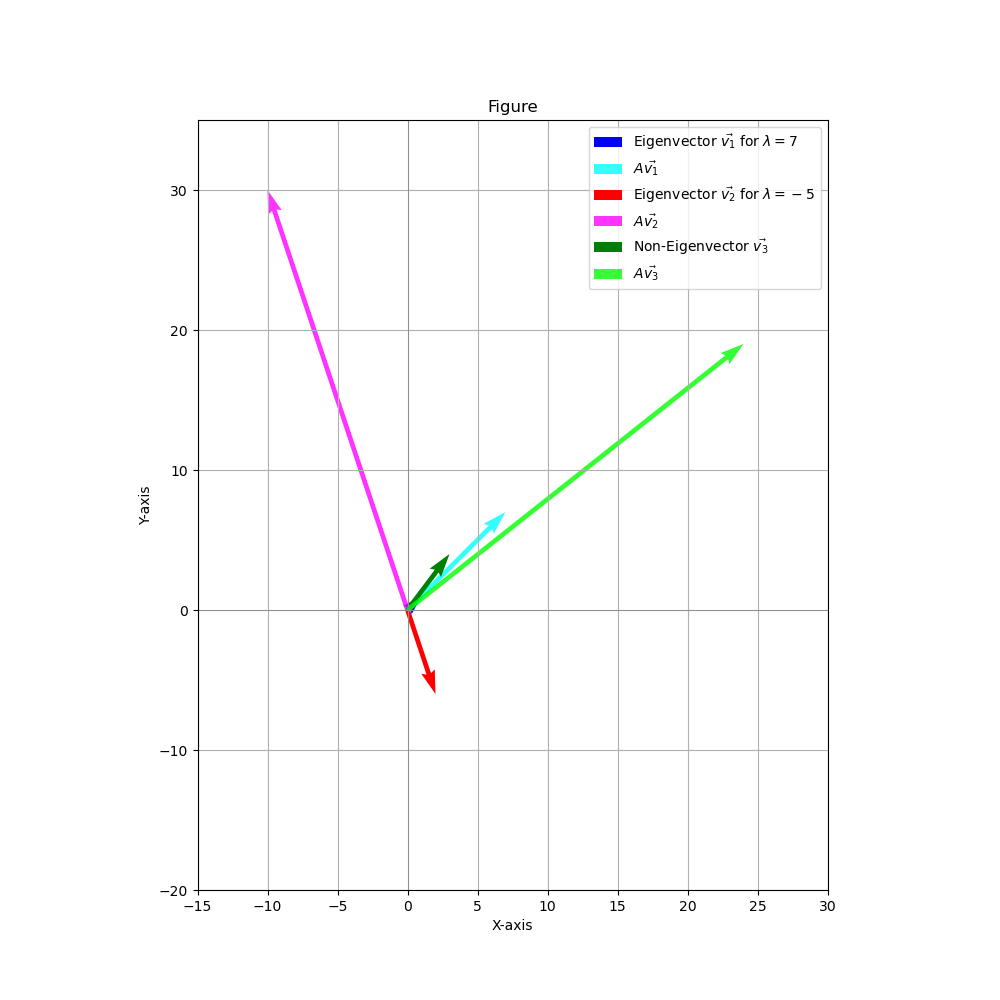
\includegraphics[width=\columnwidth, height=0.8\textheight, keepaspectratio]{figs/figure1.png}
        \end{center}
    \end{frame}
    
    \end{document}